\begin{enunciado}{\ejExtra}{\tiny[\violet{recu 5/12/2024}]}
  Sean $p_1 = (1, 0)$ y $p_2 = (1,1)$ dos puntos en $\reales^2$.
  \begin{enumerate}[label=(\alph*)]
    \item Hallar la recta que pasa por el origen (es decir, $y = \alpha x$) que mejor aproxima a los
          puntos $p_1$ y $p_2$ en el sentido de cuadrados mínimos. Calcular el error cometido en la aproximación.

    \item Sea $y = \tilde{\alpha}x$ la recta hallada en el ítem anterior. Probar que $y = \tilde{\alpha}x$ es la
          recta que pasa por el origen que mejor aproxima en el sentido de cuadrados mínimos a los puntos $p_1 = (1, -\beta/2)$
          y $p_2 = (1, 1+ \beta/2)$ para cualquier $\beta \en \reales$. ¿El error cometido es el mismo que en el ítem anterior?
          Justificar.
  \end{enumerate}

\end{enunciado}
\begin{enumerate}[label=(\alph*)]
  \item Minimizar en el sentido de cuadrado mínimos:
        $$
          \sumatoria{i = 1}{2} (y_i - \alpha x_i)^2 =
          \ub{
            (y_1 - \alpha x_1)^2 + (y_2 - \alpha x_2)^2
          }{
            \norma{\bm{y} - \alpha \bm{x}}_2^2
          }
          \flecha{minimizar}[el sistema]
          \minimo(\norma{\bm{y} - \alpha \bm{x}}_2^2)
        $$
        Ecuaciones normales:
        $$
          \ub{
            \matriz{cc}{
              1 & 1
            }
          }{
            A^t
          }
          \ub{
            \matriz{c}{
              1\\
              1
            }
          }{
            A
          }
          \alpha
          =
          \ub{
            \matriz{cc}{
              1 & 1
            }
          }{
            A^t
          }
          \ub{
            \matriz{c}{
              0\\
              1
            }
          }{
            y
          }
          \sii
          2 \alpha = 1
          \sii
          \alpha = \frac{1}{2}
        $$
        La recta que pasa por el origen y que mejor aproxima es:
        $$
          \cajaResultado{
            y = \frac{1}{2}
          }
        $$
        El error cometido al usar la recta $y = \frac{1}{2}x$ para aproximar los puntos $p_1$ y $p_2$:
        $$
          \varepsilon = \norma{
            \sumatoria{i = 1}{2} (y_i - \red{\frac{1}{2}} x_i)^2
          }_2^2
          =
          \norma{\bm{y} - \red{\frac{1}{2}} \bm{x}}_2^2 =
          \norma{
            \matriz{c}{
              0\\
              1
            }
            -
            \red{\frac{1}{2}}
            \matriz{c}{
              1\\
              1
            }
          }_2^2 =
          \norma{
            \matriz{c}{
              -\frac{1}{2}\\
              \frac{1}{2}
            }
          }_2^2 =
          \frac{1}{2}
          \sii
          \cajaResultado{
            \varepsilon = \frac{1}{2}
          }
        $$
        El error se puede apreciar en el gráfico como el área de esos dos cuadrados que tienen de lado $\frac{1}{2}$, al sumarlas se obtiene el $\varepsilon$.
        $$
          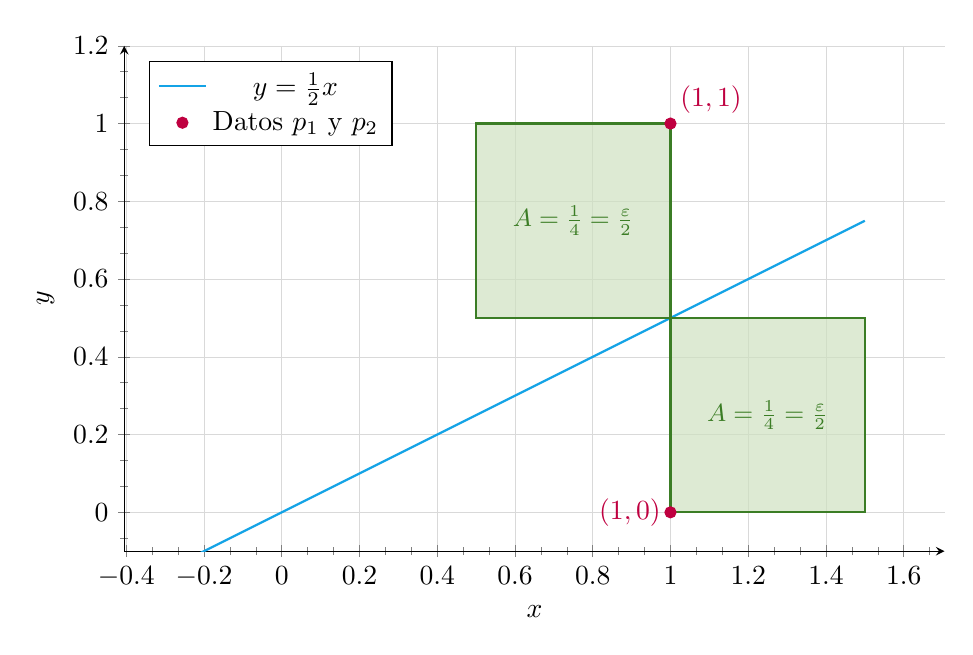
\begin{tikzpicture}
            \begin{axis}[
                axis lines = left,
                axis equal,
                xlabel = {$x$},
                ylabel = {$y$},
                xmin = -0.2, xmax = 1.5,
                ymin = -0.1, ymax = 1.2,
                grid = major,
                grid style = {very thin, gray!30},
                minor tick num = 2,
                minor grid style = {very thin, gray!15},
                width = 12cm,
                height = 8cm,
                samples = 100,
                smooth,
                legend pos = north west
              ]

              \addplot[
                domain=-0.5:1.5,
                Cerulean,
                thick
              ] {0.5 * x};

              \fill[OliveGreen!20, opacity=0.7] (axis cs:1,1) rectangle (axis cs:0.5,0.5);
              \draw[OliveGreen, thick,line cap=rect] (axis cs:1,1) rectangle (axis cs:0.5,0.5);
              \node[OliveGreen, font=\small] at (axis cs:0.75,0.75) {$A = \frac{1}{4} = \frac{\varepsilon}{2}$};

              \fill[OliveGreen!20, opacity=0.7] (axis cs:1,0) rectangle (axis cs:1.5,0.5);
              \draw[OliveGreen, thick,line cap=rect] (axis cs:1,0) rectangle (axis cs:1.5,0.5);
              \node[OliveGreen, font=\small] at (axis cs:1.25,0.25) {$A = \frac{1}{4} = \frac{\varepsilon}{2}$};

              \addlegendentry{$y = \frac{1}{2} x$}

              \addplot[
                only marks,
                mark = *,
                mark size = 2pt,
                purple
              ] coordinates {
                  (1, 0)
                  (1, 1)
                };
              \addlegendentry{Datos $p_1$ y $p_2$}

              \node[left, purple] at (axis cs:1,0) {$(1, 0)$};
              \node[above right, purple] at (axis cs:1,1) {$(1, 1)$};
            \end{axis}
          \end{tikzpicture}
        $$

  \item
        Con los puntos
        $p_1 = (1, -\frac{\beta}{2})$, \,
        $p_2 = (1, 1 + \frac{\beta}{2})$
        la simetría del ejercicio sigue siendo la misma.

        Ecuaciones normales:
        $$
          \ub{
            \matriz{cc}{
              1 & 1
            }
          }{
            A^t
          }
          \ub{
            \matriz{c}{
              1\\
              1
            }
          }{
            A
          }
          \alpha
          =
          \ub{
            \matriz{cc}{
              1 & 1
            }
          }{
            A^t
          }
          \ub{
            \matriz{c}{
              -\frac{\beta}{2}\\
              1 + \frac{\beta}{2}
            }
          }{
            y
          }
          \sii
          2 \alpha = 1
          \sii
          \alpha = \frac{1}{2}
        $$
        La recta que pasa por el origen y que mejor aproxima es nuevamente:
        $$
          \cajaResultado{
            y = \frac{1}{2}
          }
        $$
        El error cometido al usar la recta $y = \frac{1}{2}x$ para aproximar los puntos $p_1$ y $p_2$:
        $$
          \varepsilon =
          \norma{
            \matriz{c}{
              -\frac{\beta}{2}\\
              1 + \frac{\beta}{2}
            }
            -
            \red{\frac{1}{2}}
            \matriz{c}{
              1\\
              1
            }
          }_2^2 =
          \norma{
            \matriz{c}{
              - \frac{1 + \beta}{2}\\
              \frac{1 +\beta}{2}
            }
          }_2^2 =
          \frac{(1 + \beta)^2}{2}
          \sii
          \cajaResultado{
            \varepsilon = \frac{(1 + \beta)^2}{2}
          }
        $$
\end{enumerate}

\begin{aportes}
  \item \aporte{\dirRepo}{naD GarRaz \github}
\end{aportes}
